\begin{frame}[hasprev=false,hasnext=true]
\label{example:ariane-5}
\frametitle{Ariane 5}
\framesubtitle{Description}

\begin{itemize}
	\item Ariane 5 is an expendable launch system used to deliver payloads into
	geostationary transfer orbit or low Earth orbit.

	\item The rocket took a decade to be developed and required 7 billions
	dollars.
\end{itemize}

\begin{figure}
	\centering
	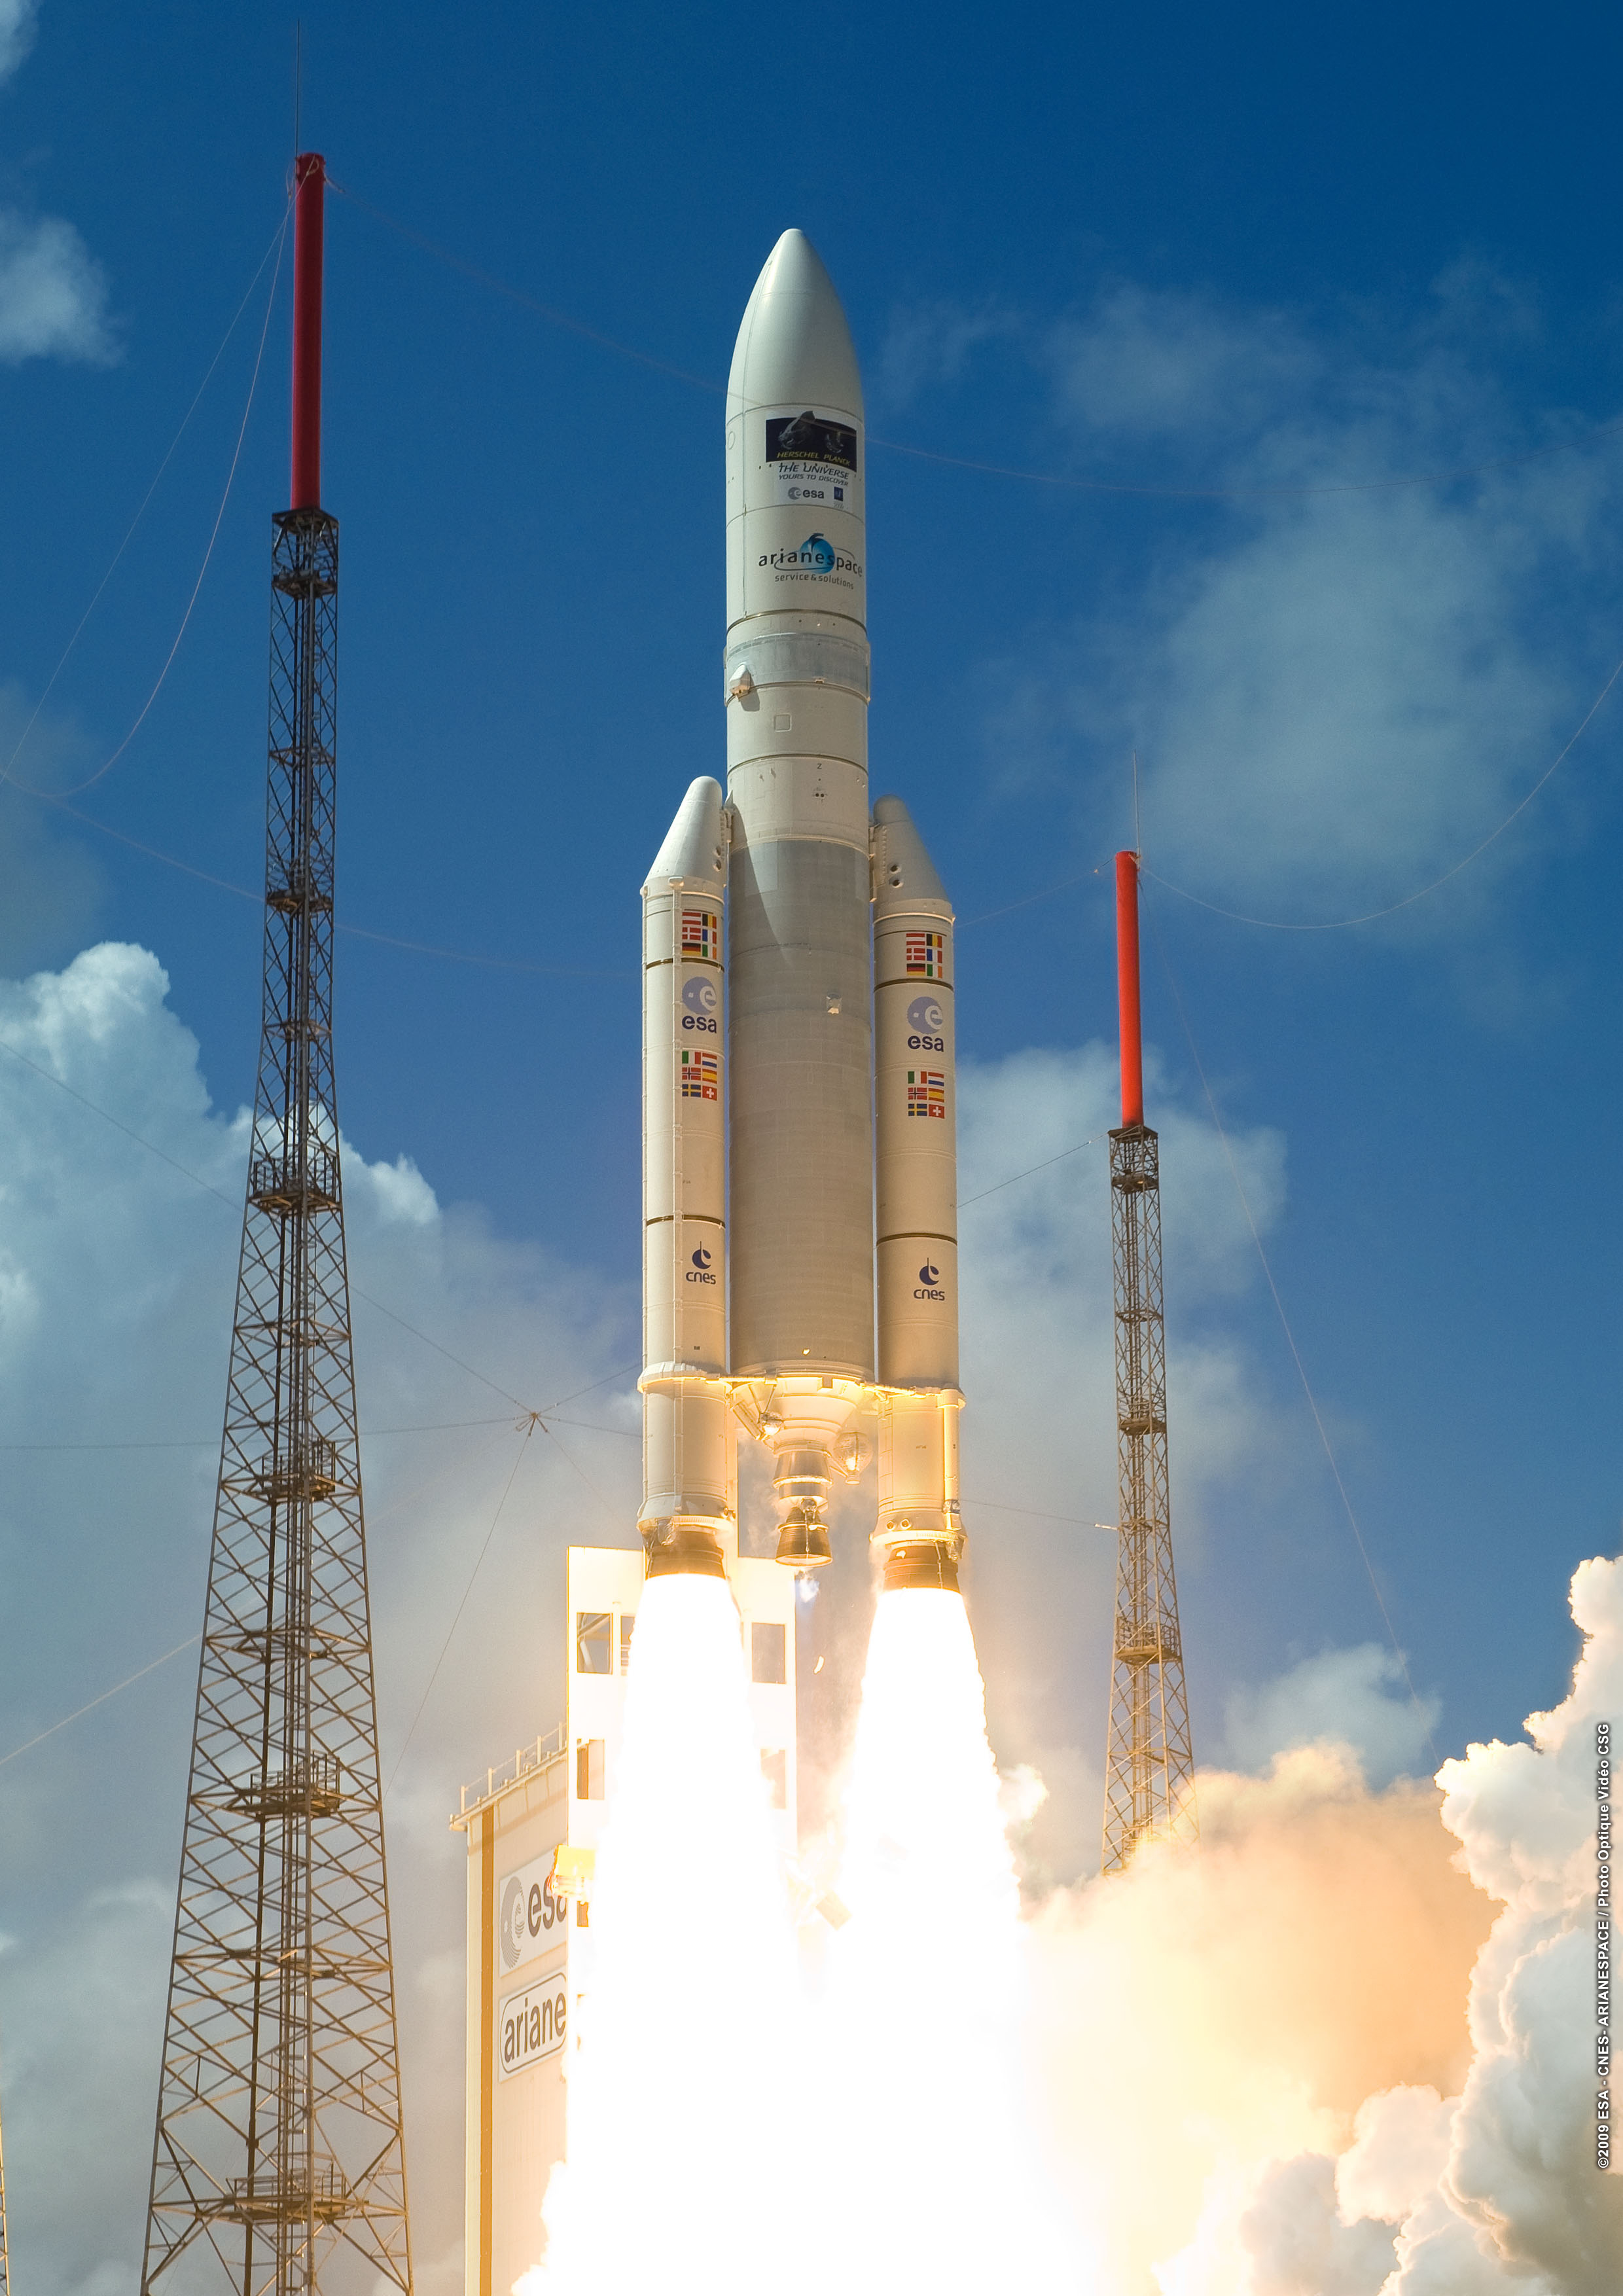
\includegraphics[width=.4\textwidth]{aux/examples/ariane-5/ariane-5}
\end{figure}
\end{frame}


\begin{frame}[hasprev=true,hasnext=true]
\frametitle{Ariane 5}
\framesubtitle{Problem}

\begin{itemize}
	\item On 4 June 1996, the maiden flight of the Ariane 5 launcher ended in a
	failure.

	\item Only about 40 seconds after initiation of the flight sequence, at an
	altitude of about 3700 m, the launcher veered off its flight path, broke up
	and exploded.
\end{itemize}

\begin{figure}
	\centering
	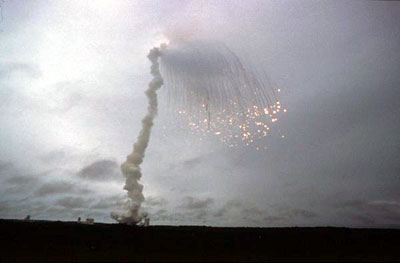
\includegraphics[width=7.5cm]{aux/examples/ariane-5/ariane-5-self-destruction}
\end{figure}
\end{frame}


\begin{frame}
\frametitle{Ariane}[hasprev=true,hasnext=false]
\framesubtitle{Diagnostic}

\begin{itemize}
	\item The back-up Inertial Reference System failed, followed immediately by
	the failure of the active Inertial Reference System.

	\item The failure cause was a fault in the software that calculated the
	horizontal velocity of the rocket.
	\begin{itemize}
		\item The variable that stored the value was 64 bit wide (floating
		point) and was incorrectly changed to 16 bits (signed integer).

		\item The value was bigger than 32,767 (biggest value a signed integer
		can represent), causing a conversion failure.
	\end{itemize}

	\item Insufficient testing for components reused from Ariane 4 were the
	cause of the failure.
\end{itemize}
\end{frame}